\documentclass{aastex63}
\usepackage{amsmath}
\newcommand{\be}{\begin{eqnarray}}
\newcommand{\ee}{\end{eqnarray}}
\def\la{\mathbin{\lower 3pt\hbox
      {$\rlap{\raise 5pt\hbox{$\char'074$}}\mathchar"7218$}}}
\def\ga{\mathbin{\lower 3pt\hbox
      {$\rlap{\raise 5pt\hbox{$\char'076$}}\mathchar"7218$}}} %> or of order
\renewcommand{\vec}[1]{\mathbf{#1}}
%\renewcommand{\vec}[1]{\ensuremath{\boldsymbol{#1}}} %boldface vector style
\newcommand{\grad}{\mathbf{\nabla}}
\newcommand\lya{Ly$\alpha$\ }

%%% FOR DRAFTING: REMOVE AFTER PAPER IS COMPLETE!
\usepackage{xcolor}
\newcommand{\todo}[1]{\textcolor{red}{#1}}
\newcommand{\proposed}[1]{\textcolor{blue}{#1}}

\received{}
\revised{}
\accepted{\today}
\submitjournal{APJ}


\shorttitle{Resonant Scattering of \lya}
\shortauthors{McClellan et al.}

\graphicspath{{./}{figures/}}


\begin{document}

\title{Resonant Scattering in a Uniform Sphere with Large Optical Depth}



\correspondingauthor{B. Connor McClellan}
\email{bcm2vn@virginia.edu}

\author{B. Connor McClellan}
\author{Shane Davis}
\author{Phil Arras}
\affiliation{Department of Astronomy, University of Virginia, Charlottesville, VA 22904, USA}


\begin{abstract}

The solution of the radiative transfer equation for resonant scattering of Lyman $\alpha$ photons for a uniform sphere of constant gas density is found in the limit of large line center optical depth. A monochromatic source of photons is assumed at the center of the sphere, and the intensity within the sphere and at the surface is found with the Eddington approximation for the angular dependence. The solution can be represented a sum of two terms: a semi-analytic solution of the homogeneous equation which is required for the mean intensity $J=0$ at the surface, and a solution of the homogeneous equation which enforces the correct, zero-ingoing intensity boundary conditions at the surface. It is the compact, analytic form as well as the piece accounting for the correct, frequency dependent boundary condition that is novel in this study. The analytic solution is compared to numerical solutions with the Monte-Carlo method, which are valid at arbitrary optical depth, and the deviations from exact solution are investigated.

\end{abstract}


\keywords{}

\section{To Do List}
$\blacksquare$ Change all plots to use just wing line profile, exclude Doppler core

$\blacksquare$ Use larger n phot MC runs for tau=1e5

$\blacksquare$ Remove details about $H_d$, change wording in abstract and derivations

$\square$ Add eigenmodes plots

$\square$ Add discussion of numerical solution of time-dependent equations

$\square$ Add results, summary, conclusions, etc

\section{Introduction} 
\label{sec:intro}

The outer layers of planetary atmospheres are central to a planet's evolution, since they can shelter the lower atmosphere from high energy radiation and regulate the escape of gas into space. In atmospheres with thick layers of atomic hydrogen, stellar Lyman Alpha (Ly$\alpha$) radiation is especially important in this process as the optical depth at line center is large. Ionization and subsequent recombination can generate \lya within the planet's atmosphere, dissociating molecules in lower layers and causing heating by collisional de-excitation. \lya can also excite H atoms to the 2p state, creating a population of Balmer-line absorbers that can be observed via transmission spectroscopy.

%There's a much thicker layer of atomic hydrogen
%It's a very optically thick region
% Care about lya going into the planet's atmosphere and dissociating molecules
% Observational: observe the transits in lyman alpha
%Chen liang's paper - focus on the section where he shows the results of the lya transfer - can cause heating deeper in the atmosphere, collisional de-excitation. Summarize some of the things that lya does to the atmosphere. Ionize low ionization-potential atoms (<10.2 eV)
%Large Lya line intensity, lots of H atoms, then lya is constantly exciting and de-exciting. Then, n=2 is populated so Balmer lines can also be absorbed. This explains why strong balmer absorption is observed in transits to begin with. Otherwise, you would need very high temperatures to populate the n=2 state.
% Focus on later sections, especially balmer absorption near the end of the paper.

% Put emphasis on the fact that Lya is generated within the atmosphere --- ionization balanced by recombination, rate equilibrium. Recombination gives you lyman alpha again. Collisions decrease the density in the 2s states. The efficiency of producing lya is quite high, and that's immediately at high optical depth.

Hubble Space Telescope (HST) observations with STIS have found large \lya transit depths around a handful of exoplanets, indicating an extended distribution of hydrogen: \citet{2003Natur.422..143V, 2012A&A...543L...4L, 2012A&A...547A..18E, 2015Natur.522..459E,  2017A&A...597A..26B, 2017A&A...599L...3B, 2017A&A...602A.106B, 2018A&A...620A.147B, 2019AJ....158...50W, 2019EPSC...13.1928L, 2020ApJ...888L..21G,2021arXiv210309864B}. These observations have revealed a population of atoms extending out to distances of order the planetary radius for several planets around bright, nearby stars, motivating a study of the physics of \lya interactions with H atoms surrounding a planet. The importance of the \lya line in the atmospheric dynamics of these systems necessitates a careful treatment of resonant scattering in order to construct accurate models of atmospheric heating and escape. However, the extreme optical depths at \lya line center introduce a computational barrier to simulating radiative transfer via Monte Carlo methods.

The main impediment to performing magnetohydrodynamic simulations with fully a coupled radiative transfer solution via Monte Carlo methods is the prohibitive computational cost. A primary factor in the cost of Monte Carlo is that the number of scatterings a photon undergoes is proportional to the line center optical depth.  Near the base of the atmosphere, individual simulation cells can have optical depths of more than a million, so most of the time is spent integrating photons in these cells. This means that any method that can treat these zone via an analytic solution has the potential to greatly accelerate the calculation.

There are several methods that are commonly used to accelerate Monte Carlo radiation transfer calculations.  The simplest class of methods that is specific to resonance line transfer are core skipping methods \citep{1968ApJ...153..783A,2002ApJ...567..922A}.  These methods focus on Monte Carlo transfer in the wings of the line and avoid scatterings in the core. Line core photons are pushed to the wings by biasing the atomic velocity distribution to high velocities so the opacity is lower and escape is more rapid.

A second class of methods are hybrid diffusion methods \citep{2001JCoPh.172..543G}, such as discrete diffusion Monte Carlo \citep{2007JCoPh.222..485D}. This involves designating sufficiently optically thick simulations cells for computation via a finite difference representation of the radiation transfer equation. This method is particularly attractive for gray opacity applications where a single diffusion equation can be computed.  For the resonant scattering problem, where the opacity is a strong function of frequency, implementation of this method is more complex and computationally demanding as it requires the solution of many frequency groups, but can lead to a considerable speed up \citep{2018MNRAS.479.2065S}.

A third class of methods are modified random walk methods \citep{1984JCoPh..54..508F,2009A&A...497..155M, 2010A&A...520A..70R}. In this case a spherical volume (usually the largest within a simulation cell) is chosen when the scattering mean-free-path is small compared with the zone size.  An outgoing photon is then randomly sampled on the surface of this outgoing sphere by drawing its properties from distributions in outgoing frequencies, directions and escape times, based on solutions to the diffusion equation within a uniform sphere. A method similar to this has been applied by \citet{2006ApJ...645..792T} to Lyman $\alpha$ transfer using the \cite{1990ApJ...350..216N} solution.

The need for accurate distributions from which to draw outgoing photon properties motivates this work; namely, an analytic solution to the steady-state problem of \lya resonant scattering in spherical geometry. In addition, a semi-analytic solution to time-dependent \lya diffusion through the same medium is explored to quantify how long the photons are expected to spend in the domain before escaping. These solutions will be shown to accurately represent the photon distributions in frequency and time-to-escape at the surface of a spherical volume of gas, highlighting their potential for use as a Monte Carlo accelerant in magnetohydrodynamic calculations of phenomena involving \lya resonance-line radiation.

\section{ previous analytic work }

\citet{1973MNRAS.162...43H, 1974MNRAS.166..373H} demonstrated that resonance-line radiation transfer in low-density, optically-thick media can be described by the Poisson equation. However, the accuracy of their solution is limited by the treatment of the boundary conditions. In their eigenfunction expansion, the spatial and frequency components of the differential equation are separated, yet the spatial eigenvalues are defined as being explicitly frequency-dependent. The resulting solution for large optical depths would suggest the mean intensity at the boundary of the slab is zero, which is unphysical. A more detailed discussion of the boundary condition is included in Section \ref{sec:steadystate}. \citet{1990ApJ...350..216N} follows this approach in an attempt to extend the result to media of intermediate optical depth, including the effects of scattering in the Doppler core of the line, but again does not use the correct boundary condition. \citet{?} improved on this approach, producing a divergent, inhomogeneous solution to the problem in 1D slab geometry that includes the effect of photon absorption within the medium. \citet{2006ApJ...649...14D} generalize the problem to spherical geometry, which is the same physical set up used here. Following this, \citet{2020arXiv200509692L} presents closed-form solutions for the radiation field in spherical geometry, utilizing the ``core skipping'' method discussed in \citet{2015MNRAS.449.4336S} to handle photon frequency redistribution within the Doppler core. This technique involves drawing the atom's velocity from a truncated Gaussian distribution, forcing photons back into the wing when they scatter into the core. This is motivated by the assumption that all core scattering results in zero spatial diffusion until the photon is redistributed back out into the wing where the mean free path becomes much larger and it can diffuse in space again. However, it is not clear whether this prescription is fully independent of the choice of velocity distribution.

Radiation forces due to \lya transfer have been calculated in \citet{1976ApJ...208..286W} in plane-parallel geometry. However, these solutions are limited to optical depths below $2.5 \times 10^3$. In the grid cells of a radiation magnetohydrodynamic simulation that includes resonant scattering, for example, it would be necessary to calculate the radiation force on each cell face due to \lya at line center optical depths of up to 1 million. A discussion of Monte Carlo code acceleration for optical depths as large as these in a uniform, plane-parallel medium with no absorption is presented in  \citet{2002ApJ...567..922A,2015MNRAS.449.4336S}. In terms of the time dependence, \citet{1994ApJ...427..603R} introduce an ansatz for the Fokker-Planck diffusion equation in order to quantify the relaxation timescale necessary to reach a quasi-static solution. Notably, the full Voigt function is used for the line profile rather than restricting scattering to the damping wing only.


\section{STEADY-STATE SOLUTION}
\label{sec:steadystate}

Two solutions will be considered for this problem.

\begin{enumerate}
    \item a \textbf{J=0 solution} ($\rm H_0$) which includes the delta function solution at the source and satisfies $J=0$ at $r=R$,
    \item the \textbf{bc solution} ($\rm H_{bc}$) that allows the boundary condition $J=\sqrt{3}H$ to be satisfied.
\end{enumerate}

\noindent The full solution is the sum of the $J=0$ solution and the bc solution. The problem is as follows. The radiative intensity $I = dE/(dA dt d\Omega d\nu)$ is the energy per perpendicular area $dA$, per time $dt$, per solid angle $d\Omega$ and per frequency $d\nu$ \citep{1986rpa..book.....R}. Here the time-dependence of $I$ has been ignored, which assumes the fluid is changing on timescales long compared to a light-crossing time. The intensity $I=I(\vec{x},\vec{n}, \nu)$ will be considered a function of position $\vec{x}$, photon (unit) direction vector $\vec{n}$, and cyclic frequency $\nu$. In the Eddington and two-stream approximations, $I(\vec{x},\nu) \simeq J(\vec{x},\nu) + 3 \vec{n} \cdot \vec{H}(\vec{x},\nu)$, where $J=(1/4\pi) \int d\Omega I$ is the mean intensity and $\vec{F} = 4\pi \vec{H}= \int d\Omega \vec{n} I$ is the flux.  

Photons of frequency $\nu$ near line center frequency $\nu_0$ are considered. The Doppler width will be written $\Delta = \nu_0 v_{\rm th}/c$, where $v_{\rm th}=\sqrt{2k_{\rm B}T/m_{\rm H}}$ is the thermal speed of hydrogen atoms of mass $m_{\rm H}$ and temperature $T$, and $c$ is the speed of light. The photon frequency in Doppler units will be written $x = (\nu-\nu_0)/\Delta$. For upper-state de-excitation rate $\Gamma$, the ratio of natural to Doppler broadening is $a=\Gamma/(4\pi \Delta)$. 
The transfer equation is \citep{1986rpa..book.....R}
\be
\frac{1}{c} \frac{\partial I}{\partial t} + \vec{n} \cdot \grad I & =& - \left( \alpha_{\rm sc} + \alpha_{\rm abs} \right) I + (1-p) j_{\rm sc} + j_{\rm em}.
\label{eq:rteqn}
\ee
The scattering coefficient, or inverse mean free path to scattering, is 
\be
\alpha_{\rm sc} & = & n_{\rm sc}\, \frac{\pi e^2}{m_e c}\, f\, \frac{H(x,a)}{\sqrt{\pi} \Delta}
= k \phi   
\ee
where $n_{\rm sc}$ is the number density of scatterers, $e$ and $m_e$ are the charge and mass of the electron, $f$ is the oscillator strength of the transition, $H(x,a)$ is the Voigt function, $k = n_{\rm sc} (\pi e^2/m_e c) f$, and the Voigt line profile is $\phi = H(x,a)/(\sqrt{\pi} \Delta)$, which is normalized as $\int d\nu\, \phi(\nu) = 1$. The absorption coefficient $\alpha_{\rm abs}$, or inverse mean free path to true absorption, is a sum over number density of the absorber times absorption cross section. Once the incoming photon has promoted the electron to an excited state, the collisional de-excitation probability is $p$, and hence only a fraction $1-p$ of the excitations lead to re-emission of photons.


\subsection{Derivation of the Steady-State Solution}
Now, consider a sphere of radius $R$ and uniform density, with line-center optical depth $\tau_0 = (k/\sqrt{\pi}\Delta)R$. After changing variables from $\nu$ to $\sigma$ using $d\sigma = \sqrt{2/3}d\nu/(\Delta^2 \phi)$ in Eq. \ref{eq:rteqn} and performing all angular integrals, we obtain Eq. \ref{eq:finaleqn} (see Appendix \ref{app:rteqn_derivation}) and set $p=\alpha_{\rm abs}=0$ to eliminate photon destruction terms. With a photon emission term given by Eq. \ref{eq:jem}, this gives the transfer equation
\be
\nabla^2 J + \left( \frac{k}{\Delta} \right)^2 \frac{\partial^2 J}{\partial \sigma^2} & = & 
- \frac{ \sqrt{6} kL}{4\pi \Delta^2} \delta^3(\vec{x} - \vec{x}_s) \delta (\sigma - \sigma_{\rm s})
\label{eq:rt_no_destr}
\ee
where the form of the source term is in Eq. \ref{eq:jem_v2}. The boundary condition is that there is no incoming flux at the surface, which can be written
\citep{1986rpa..book.....R}
\be
J & = & \sqrt{3} H
\label{eq:bc}
\ee
at $r=R$. An analytic solution $J_d$ which is divergent at the center of the sphere and at the emission frequency may be found. However, it is not a good approximation to the true solution, as it is too large at $r=R$ by a factor of $J_{\rm d}(R,\sigma)/ H_{\rm d}(R,\sigma) \sim a\tau_0/x^2 \sim (a\tau_0)^{1/3} \gg 1$. This solution is included in Fig. \ref{fig:sol_mc_residual_0} for qualitative understanding, but will not be discussed further.

A better approximation to the true solution has been derived by \citet{2006ApJ...649...14D}, who generalized the closed-form solution in slab geometry found in \citet{1990ApJ...350..216N}. They found a closed-form solution which satisfies a $J=0$ boundary condition at $r=R$. We generalize their solution to allow emission at frequency $\nu_{\rm s}$ away from line center. The result is
\be
J_0 & = & \left( \frac{\sqrt{6}L}{32\pi^2 \Delta} \right)
\left( \frac{1}{Rr} \right)
\left( 
\frac{ \sin(\pi r/R) }{ \cosh \left[ \frac{\pi \Delta}{k R} (\sigma - \sigma_{\rm s}) \right] - \cos(\pi r/R)}
\right)
\label{eq:J0}
\ee
and
\be
H_0 & = & \left( \frac{1}{3k\phi} \right)
\left( \frac{\sqrt{6}L}{32\pi^2 \Delta} \right)
\left( \frac{1}{Rr^2} \right)
\left( 
\frac{ \sin(\pi r/R) }{ \cosh \left[ \frac{\pi \Delta}{k R} (\sigma - \sigma_{\rm s}) \right] - \cos(\pi r/R)}
\right. \nonumber \\ & & \left. - \left( \frac{\pi r}{R} \right)
\frac{ \cos(\pi r/R) }{ \cosh \left[ \frac{\pi \Delta}{k R} (\sigma - \sigma_{\rm s}) \right] - \cos(\pi r/R)}
+ \left( \frac{\pi r}{R} \right)
\frac{ \sin^2(\pi r/R) }{ \left[ \cosh \left[ \frac{\pi \Delta}{k R} (\sigma - \sigma_{\rm s}) \right] - \cos(\pi r/R) \right]^2 }
\right).
\label{eq:H0}
\ee
Again $J_0 \gg H_0$, except very near the $r=R$, where it goes to zero. The flux at $r=R$ can be written
\be
H_0(R, \sigma) & = & \left( \frac{1}{3k\phi} \right)
\left( \frac{\sqrt{6}L}{32\pi \Delta} \right)
\left( \frac{1}{R^3} \right)
\left( 
\frac{ 1 }{ \cosh \left[ \frac{\pi \Delta}{k R} (\sigma - \sigma_{\rm s}) \right] +1 }
\right).
\label{eq:H0surf}
\ee
Eq. \ref{eq:H0surf} will be shown to be a much better approximation to the solution, which is valid near the delta function at the center, and is a much better approximation at the surface. It is still only a good approximation near line center at the surface. It decreases exponentially rather than as a power-law in frequency, giving a much smaller flux on the line wings as compared to the divergent solution. 

The question is how to satisfy the surface boundary condition in Eq. \ref{eq:bc}. On this point, we note that the derivation in \citet{1973MNRAS.162...43H}, and numerous studies later studies, does not actually produce a valid solution of the transfer equation and boundary condition. The reason is as follows. In the notation of \citet{1973MNRAS.162...43H}, a separation of variables
$J(\tau,\sigma) = \theta(\tau) j(\sigma)$ in spatial variable $\tau$ and frequency variable $\sigma$ is attempted (their Equations 16 and 23). The solutions for the eigenfunctions $\theta(\tau)$ and $j(\sigma)$ then depend explicitly on the separation constant $\lambda$. In order to satisfy the boundary conditions, the separation constant must satisfy an eigenvalue equation of the form
\be
\lambda \tan(\lambda B) & = & \frac{3}{2} \phi,
\label{eq:evalue}
\ee
where $2B$ is the slab optical depth at line center, and $\phi$ is the line profile ($\Delta \phi(\nu)$ here). The key point is that the line profile depends on one of the coordinates, frequency, and this causes the eigenvalues of the separation constant to depend on frequency. But then the separation constant is not constant, and it does not satisfy Eq. \ref{eq:rt_no_destr} since the frequency derivatives will act on the separation ``constant", giving extra terms. To our knowledge the errors introduced by this ansatz have never been quantified. 

In the limit of large optical depth $B$, \citealt{1973MNRAS.162...43H} approximates the eigenvalues as $\lambda_n B \simeq \pi (n-1/2)$, which gives $J=0$ at the surface. This is essentially the result in Eq. \ref{eq:J0} above. However, since this solution gives zero at the surface, their Eq. 34 subsequently allowed the separation constant to have a small deviation from the above expression, which was explicitly frequency dependent. This allowed a nonzero intensity at the surface, but at the cost of rendering the separation of variables assumption invalid. 

% Dijkstra
%Despite this treatment, a calculation of the surface flux from their Eq. 13 compared with the total emerging flux density at the surface of the sphere (Eq. C17) yields a $J=2H$ surface boundary condition. However, under the two-stream approximation, a surface boundary condition $J=\sqrt{3}H$ is necessary to properly normalize the radiation pressure.

A different solution method is attempted here: namely, a continuous Fourier expansion in the frequency variable $\sigma$. The full solution is written
\be
J(r,\sigma) & = & J_0(r,\sigma) + J_{\rm bc}(r,\sigma)
\ee
and
\be \label{eq:totalflux}
H(r,\sigma) & = & H_0(r,\sigma) + H_{\rm bc}(r,\sigma).
\ee
Here, $J_0$ and $H_0$ are the solutions of the homogeneous equation, given in Equations \ref{eq:J0} and \ref{eq:H0}. The additional term $J_{\rm bc}$ must then be a solution of the homogeneous equation
\be \label{eq:diffeq}
\frac{\partial^2J}{\partial r^2} + \frac{2}{r} \frac{\partial J}{\partial r}
+ \left( \frac{k}{\Delta} \right)^2 \frac{\partial^2 J}{\partial \sigma^2} &= & 0
\ee
with no delta function source term, and it must allow the boundary conditions to be satisfied at the surface. Since $J_0(R,
\nu)=0$, the surface boundary condition becomes
\be
J_{\rm bc}(R,\sigma) - \sqrt{3} H_{\rm bc}(R,\sigma) & = & 
J_{0}(R,\sigma) + \frac{1}{\sqrt{3}k\phi} \frac{\partial J_{0}(R,\sigma)}{\partial r} = 
\sqrt{3} H_0(R,\sigma).
\label{eq:bc2}
\ee
Plugging in a frequency dependence $J \propto e^{is\sigma}$, for ``wavenumber" $s$, gives the equation for modified spherical Bessel functions of the first kind, $i_0(z)=\sinh(z)/z$. The solution can then be represented as
\be
J_{\rm bc}(r,\sigma) & = & 
\int_{-\infty}^\infty \frac{ds}{2\pi} e^{is\sigma} A(s) 
\frac{i_0(krs/\Delta)}{i_0(kRs/\Delta)},
\label{eq:Jbc}
\ee
where $A(s)$ is the Fourier amplitude. Plugging Eq. \ref{eq:Jbc} into Eq. \ref{eq:bc2} leads to the following equation for the Fourier amplitudes,
\be
\int_{-\infty}^\infty \frac{ds}{2\pi} e^{is\sigma} A(s)
\left[ 1 + \left( \frac{s}{\sqrt{3} \Delta \phi} \right) \left( \frac{i_0^\prime(kRs/\Delta)}{i_0(kRs/\Delta)} \right) \right]
& = & \sqrt{3} H_0(R,\sigma)
\label{eq:bc3}
\ee
where $H_0(R,\sigma)$ is given by Eq. \ref{eq:H0surf}. Discretization of Eq. \ref{eq:bc3} for frequency variables $\sigma_i$ and wavenumbers $s_j$
leads to a set of coupled linear equations for the $A(s_j)$. We use equally-spaced points $\Delta \sigma = 2\sigma_{\rm max}/(N-1)$ and $\Delta s = 2\pi/(N\Delta \sigma)$, where $N$ is the number of points for each grid and solve the resulting matrix equation. The maximum frequency is set as $\sigma_{\rm max} = {\rm constant} \times \tau_0$, for a large enough constant that  the end of the frequency grid is at such small intensities that it does not affect the solution except close to the boundaries. The number of points was increased until the solution was well-resolved near line center, and only became inaccurate near the boundaries. Given the Fourier amplitudes, $J_{\rm bc}$ is computed using Eq. \ref{eq:Jbc}, and the flux is given by
\be
H_{\rm bc}(r,\sigma) & = & \left( \frac{-1}{3k\phi} \right)
\frac{\partial J_{\rm bc}(r,\sigma)}{\partial r}
= \left( \frac{-1}{3k\phi} \right)
\int_{-\infty}^\infty \frac{ds}{2\pi} e^{is\sigma} A(s) 
\left( \frac{ks}{\Delta} \right) 
\left( \frac{i_0^\prime(krs/\Delta)}{i_0(kRs/\Delta)} \right).
\label{eq:Hbc}
\ee
The Bessel functions are finite at the center and rise steeply toward the surface when $kRs/\Delta \gg 1$. 

\subsection{Scaling with Line Center Optical Depth}
To examine the relative size of the corrective term $H_{\rm bc}$ as compared to $H_0$, we consider the case where the optical depth is large and thus the mean intensity will be considerably larger than the surface flux. Starting from Eq. \ref{eq:bc2}, we assume $H_{\rm bc} \ll J_{\rm bc}$ such that
\be
J_{\rm bc}(R,\sigma) & \approx & \sqrt{3} H_0(R,\sigma).
\label{eq:bc4}
\ee
The Fourier transform for $J_{\rm bc}$ at the surface becomes
\be
J_{\rm bc}(R, \sigma) \equiv \int_{-\infty}^{\infty} \frac{ds}{2\pi} e^{is\sigma} A(s)
\ee
with Fourier amplitudes
\be \label{eq:amps}
A(s) = \sqrt{3} \int_{-\infty}^{\infty} d\sigma e^{-is\sigma} H_0(R, \sigma).
\ee
Plugging the expression for $H_0$ in Eq. \ref{eq:H0surf} into Eq. \ref{eq:amps} yields an expression for the Fourier amplitudes
\be \label{eq:plugged_amps}
A(s) = \sqrt{3}\frac{1}{3k}\frac{\sqrt{6}}{32\pi}\frac{L}{\Delta R^3} \int_{-\infty}^\infty d\sigma e^{-is\sigma}\frac{1}{\phi(\sigma)}\frac{1}{1+\cosh \left[\frac{\pi \Delta}{kR} |\sigma - \sigma_i|\right]}
\ee
with
\be
\phi(\sigma) = \left(\frac{2a}{27\pi}\right)^{1/3}\frac{1}{\Delta |\sigma|^{2/3}}.
\ee
With the line center optical depth defined as
\be \label{eq:tau0}
\tau_0 = \frac{kR}{\sqrt{\pi}\Delta}
\ee
we scale the variables $\sigma$ and $s$ by $\tau_0$, now using characteristic photon frequency $\bar \sigma = \sigma / \tau_0$ and characteristic wavenumber $\bar s = s \tau_0$. Eq. \ref{eq:plugged_amps} becomes
\be
A(\bar s) = \frac{\sqrt{2}}{32\pi}\left(\frac{27\pi}{2}\right)^{1/3}\frac{L}{kR^3}\frac{\tau_0^{5/3}}{a^{1/3}}\int_{-\infty}^\infty d\bar\sigma e^{-i\bar s \bar\sigma} |\bar\sigma^{2/3}|\frac{1}{1+\cosh \left[\sqrt{\pi}|\bar\sigma - \bar\sigma_i|\right]}.
\ee
These coefficients are used to evaluate Eq. \ref{eq:Hbc} at the surface of the sphere. Dividing $H_{\rm bc}$ by $H_0$ (Eq. \ref{eq:H0surf}) yields an overall proportionality
\be \label{eq:hbc_scaling}
\frac{H_{\rm bc}(R, \sigma)}{H_0(R, \sigma)} \propto \frac{1}{(a\tau_0)^{1/3}}.
\ee
Thus, the fractional importance of the corrective frequency-dependent boundary condition term scales as the inverse cube root of the damping parameter $a$ times the line-center optical depth $\tau_0$. At very large optical depths, it is expected that the corrective term will be small, but will become increasingly important in less optically thick media. 

By replacing the differential operators in Eq. \ref{eq:rt_no_destr} with characteristic scales $R$ and $\sigma_0$ and equating the terms on the left-hand side of this equation, a dimensionless scaling relation between frequency and space emerges.
\be
\frac{J}{R^2} &=& \left(\frac{k}{\Delta}\right)^2 \frac{J}{\sigma_0^2}
\ee
Now, using Eq. \ref{eq:tau0} and the approximation $\sigma(x)=x^3\sqrt{2\pi/27}/a$ introduced in \cite{1973MNRAS.162...43H} for large $x$, we have
\be
\frac{\sqrt{2\pi/27}}{a}x_0^3 = \frac{kR}{\Delta} = \sqrt{\pi} \tau_0.
\ee
Simplifying, we obtain the proportionality
\be \label{eq:tau_peak_scaling}
x_0 &\propto& \left(a\tau_0\right)^{1/3}.
\ee
This predicts that the characteristic photon frequency in Doppler widths should scale as the cube root of the Voigt parameter $a$ multiplied by the line center optical depth $\tau_0$, indicating the location of the spectral peaks on either side of line center --- the locations where the photons most readily escape. Since our derivations were performed assuming a Lorentzian line profile (see Appendix \ref{app:rteqn_derivation}), our solutions are technically only valid far out into the line wing, where the Doppler component of the line profile is small. Since our choice of the damping parameter $a$ is constant, the solutions of the transfer equation will perform best when the peaks of the spectral energy distribution lie well outside of the Doppler core, e.g., for large optical depths. The boundary of the Doppler core is approximately where the Gaussian and Lorentzian pieces are equal:
\be
\frac{e^{-x^2}}{\sqrt{\pi}} = \frac{a}{\pi x^2}
\ee
For \lya and a hydrogen gas of temperature $T=10^4$ K, the damping parameter $a = \Gamma / (4\pi\Delta)$ is equal to $4.72\times 10^{-4}$ in CGS units. The Doppler core is then significant over the range $-4.6 < x < 4.6$. Comparing with the locations of the spectral peaks at various optical depths using Eq. \ref{eq:tau_peak_scaling}, we find that $x_0=$3.6, 7.8, 16.8 for $\tau_0=10^5, 10^6,$ and $10^7$, respectively. Therefore, solutions derived assuming a Lorentzian line profile $\phi(x) \approx a/(\pi x^2)$ are expected to fail for lower line center optical depths where the peak of the spectrum lies near the core and improve for larger optical depths where the spectral peak is well outside of the line core.
\subsection{Comparison to Monte Carlo}

%Brief description of MC code, citing Chenliang's paper. Discuss how MC works briefly, reference some papers, talk about problem setup specific to this work. Basically want to show that the MC approach in this paper is not new and doesn't need to be justified extensively.

The Monte Carlo method is used to solve the transfer equation numerically as a point of reference for these analytic solutions. For each simulation, a total of $2^{20} \approx 10^6$ photon packets are initialized at a monochromatic source frequency $x_s$ and are allowed to propagate through the medium until escaping, at which point their positions, outgoing angles, and frequencies are logged. A constant temperature of $T=10000\ \rm K$ is set for the gas. Frequency redistribution is calculated at each scattering, including the effects of recoil, to obtain the spectrum at the surface of the spherical simulation domain. Further details of the Monte Carlo simulation are discussed in \cite{2017ApJ...851..150H}.

\begin{figure}
    \centering
    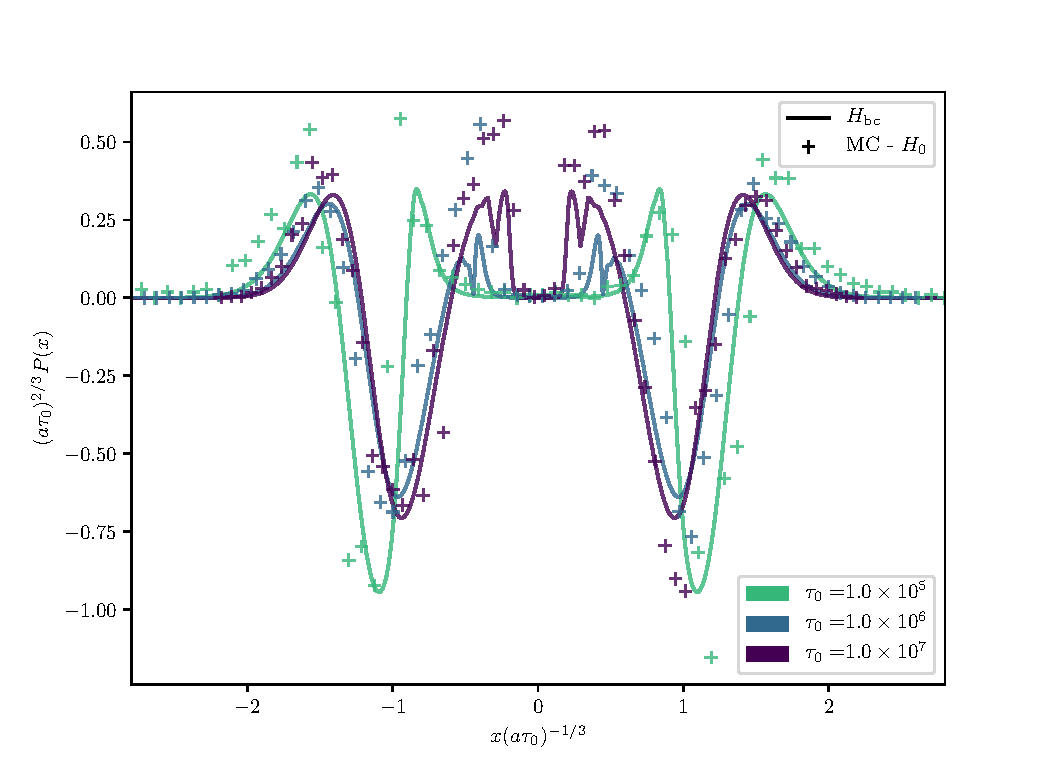
\includegraphics{taubc.pdf}
    \caption{Boundary condition term $H_{\rm bc}$ scaled by $(a\tau_0)^{1/3}$ shown for increasing line center optical depths. The Monte Carlo data minus the $H_0$ solution should be close to $H_{\rm bc}$ according to Eq. \ref{eq:totalflux}. As $\tau_0$ becomes larger, the agreement between these two improves, indicating that at large optical depths the relative size of the corrective boundary condition term scales as $(a\tau_0)^{-1/3}$}.
    \label{fig:taubc}
\end{figure}

The relative size of the boundary term $H_{\rm bc}$ with optical depth is shown graphically in Fig. \ref{fig:taubc}, where $H_{\rm bc}$ is shown for several optical depths along with Monte Carlo data. Since the Monte Carlo simulation represents the true solution, it can be compared directly against $H_{\rm bc}$ by subtracting off the homogeneous piece of the solution ($H_{\rm bc} = H - H_0$). From Eq. \ref{eq:hbc_scaling}, the size of the frequency-dependent boundary condition correction should become smaller with larger optical depths, following a $(a\tau_0)^{-1/3}$ scaling. This factor has been scaled out of the figure such that solutions for different optical depths should show close agreement if the relation holds. Indeed, agreement between $H_{\rm bc}$ and the Monte Carlo points improves as the optical depth becomes larger. At lower optical depths, the scattering of photons within the Doppler core of the line becomes important, yet our solution is not constructed to model this behavior precisely. The effects of core scattering can be seen in the Monte Carlo data, however, as the peaks of the distribution shift outward in frequency from the line core around $\tau_0 = 10^5$. Thus, the $(a\tau)^{1/3}$ scaling holds only for larger optical depths where scattering in the core can be ignored.

\begin{figure}
    \centering
    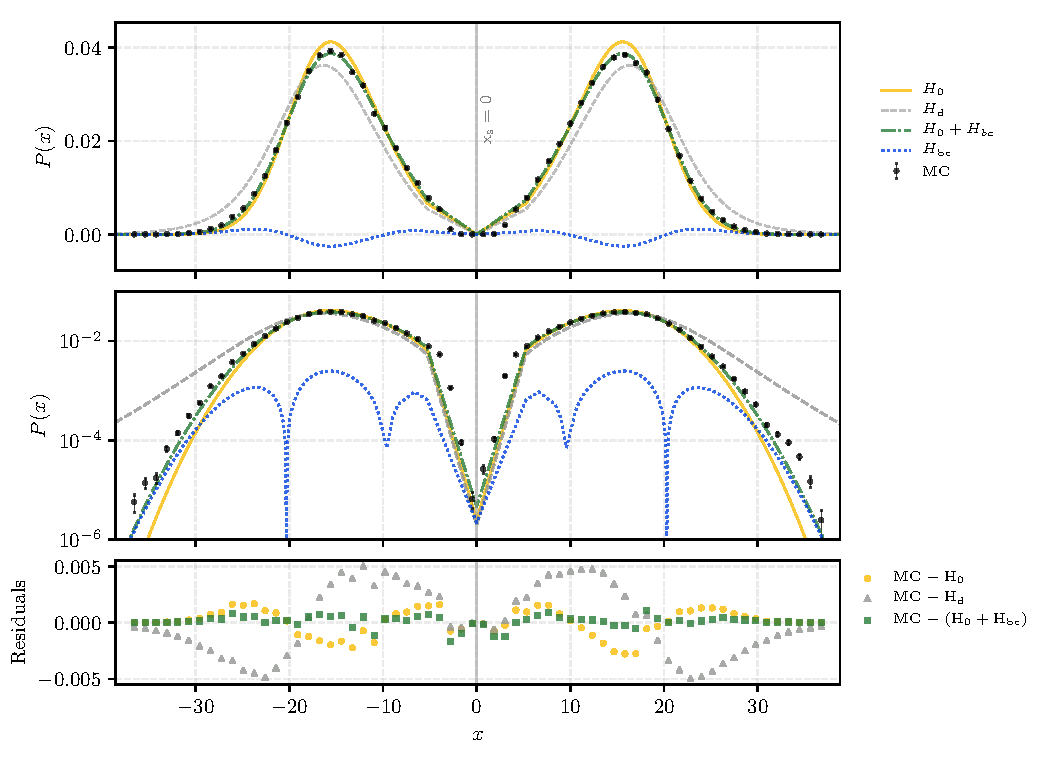
\includegraphics{final_residual.pdf}
    \caption{Analytic solution for the outgoing spectrum compared with Monte Carlo at a line center optical depth of $\tau_0 = 1 \times 10^7$. Photons are initialized with $\rm x = 0.0$. In the log-scale plot in the second panel, $|\rm H_{bc}|$ is shown instead of $\rm H_{bc}$. Residuals of each solution to the Monte Carlo data points are shown in the third panel.} 
    \label{fig:sol_mc_residual_0}
\end{figure}

We now compare each of the solutions for surface flux with Monte Carlo simulations. In Fig. \ref{fig:sol_mc_residual_0}, the Monte Carlo is shown with solutions $H_{\rm d}$, $H_{\rm 0}$, and $H_{\rm 0 + bc} = H_{\rm 0} + H_{\rm bc}$ over-plotted for an optical depth of $\tau_0 = 10^7$ and photons emitted at line center $\rm x_s = 0$. The solution with the correct frequency-dependent boundary condition enforced, $H_{\rm 0 + bc}$, has considerably lower residuals to Monte Carlo than the other solutions, especially in the line wing. It is evident that the divergent solution $H_{\rm d}$ fails in the line wings. The $H_{\rm bc}$ term, when added to the solution $H_0$ derived by \citet{2006ApJ...649...14D}, adequately corrects for the apparent excess of flux in the peaks of the spectrum. This peak excess is also present in previous work that used the \citet{1990ApJ...350..216N} solution, such as \citet{2015MNRAS.449.4336S}. The boundary term resolves the slight deficit of $H_{\rm0}$ in the line wings, further improving agreement with the numerical result. Note that as in Fig. \ref{fig:taubc} the residuals to the $H_0$ solution are a close match to the $H_{\rm bc}$ term.
 
 \begin{figure}
    \centering
    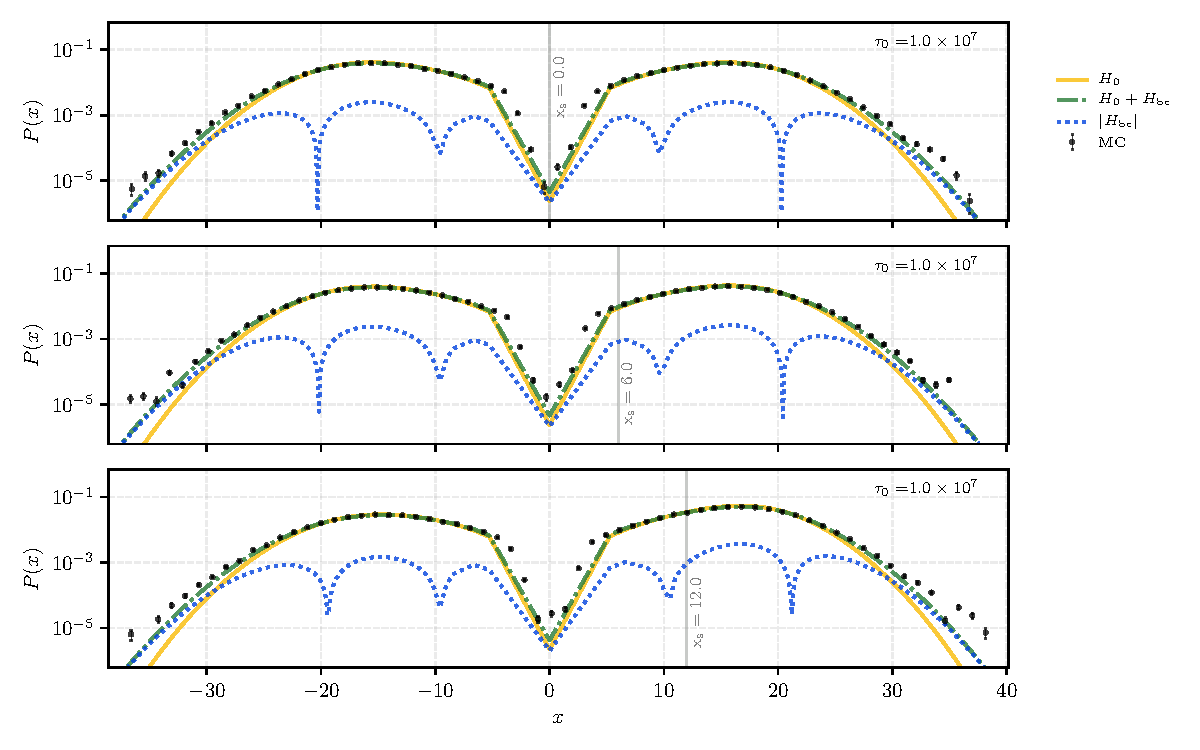
\includegraphics{xinit_threepanel.pdf}
    \caption{Analytic solution for the outgoing spectrum compared with Monte Carlo at a line center optical depth of $\tau_0 = 1 \times 10^7$. Photons are initialized with $\rm x = 0.0, 6.0, 12.0$ to examine the solutions' accuracy with a changing source frequency. TODO: Remove blue line. We really don't care about the divergent solution anymore.} 
    \label{fig:sol_mc_xinit}
\end{figure}

Since the solutions have been generalized to allow for a monochromatic source of photons at a frequency $\sigma_s$ away from line center, their agreement with Monte Carlo as a function of source frequency can also be characterized. Photons initialized closer to the line wing may travel larger mean free paths as the opacity is sensitively dependent on the line profile. The larger spatial diffusion contributes to greater escape probability, biasing the frequency distribution of escaping photons. In the limit that $|\rm x_s|$ becomes large, the distribution becomes a delta function in frequency as all photons escape the gas without scattering. Fig. \ref{fig:sol_mc_xinit} shows calculations performed for three initial photon frequencies $\rm x_s = 0.0, 6.0$, and $12.0$ for a line center optical depth of $\tau_0=10^7$. The bias in frequency distribution is slight for $\rm x_s = 6.0$ where the line profile is still relatively large, but the increase in spatial diffusion is much more substantial when photons are initialized with $\rm x_s=12.0$, further away from the line core. On this point, we note that the discrepancy between the Monte Carlo data and $H_0$ (effectively the scale of the corrective $H_{\rm bc}$ term) becomes larger as $\rm x_s$ increases. Thus, for sufficiently large optical depths and emission away from line center, the importance of enforcing frequency-dependent boundary conditions at the surface of the sphere grows. %Note: should we characterize this scaling quantitatively?

 \begin{figure}
    \centering
    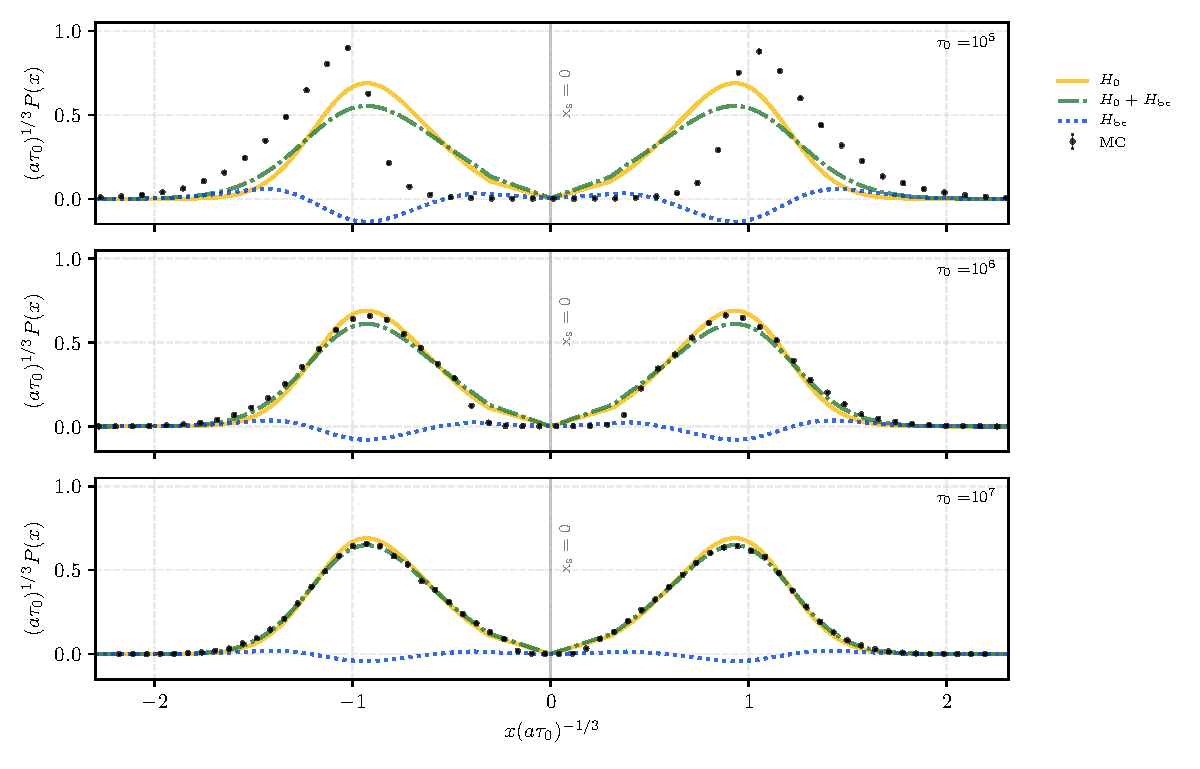
\includegraphics{tau_threepanel.pdf}
    \caption{Increasing the line center optical depth. Shown here are $\tau_0 = 10^5, 10^6, 10^7$ with the $x$ and $y$ axes scaled by the characteristic frequency diffusion scale $(a\tau_0)^{1/3}$. Photons are initialized with $\rm x = 0.0$.} 
    \label{fig:sol_mc_tau}
\end{figure}

The line center optical depth dictates the position of the peak of

\section{Time-Dependent Diffusion}
\label{sec:time_dependent}

\subsection{Background}
\label{subsec:time_dependent:background}

In order to understand the wait time distribution, the time-dependent response to an impulse is found. For simplicity a $J=0$ boundary condition will be used. This is expected to be a good approximation for $\tau_0 \gg 1$. 

\subsection{Equations}
\label{subsec:time_dependent:equations}

The source is changed to the form
\be
j_{\rm em} & = & \frac{E}{4\pi} \delta^3(\vec{x} - \vec{x}_s) \delta(\nu-\nu_{\rm s})\delta (t) .
\label{eq:jem2}
\ee
where $E$ is the energy emitted in the impulse at time $t=0$. 
The resulting equation for $J(r,\sigma,t)$ is
\be
-3 \frac{k\phi}{c} \frac{\partial J}{\partial t} + \nabla^2 J + \left( \frac{k}{\Delta} \right)^2 \frac{\partial^2 J}{\partial \sigma^2}
& = & - \frac{\sqrt{6} kE}{4\pi \Delta^2} \delta(\vec{x}) \delta (\sigma - \sigma_s ) \delta (t).
\label{eq:diffusion_eqn}
\ee

We employ an expansion in terms of spherical Bessel functions in $r$ and transform the time dependence into an imaginary frequency variable $\omega$. The eigenvalues $i\omega$ are real and positive for damped solutions to the time-dependent equation. The expansion for $J(r, \sigma, t)$ is

\be
\label{eq:jrsigmat_expansion}
J(r, \sigma, t) = -\sum_{n=1}^{\infty} \int \frac{d\omega}{2\pi} e^{-i\omega t} j_0\left(\kappa_n r\right) J(n, \sigma, \omega).
\ee

with

\be
J(n, \sigma, \omega) = \frac{2\kappa_n^2}{R} \int_0^R dr\ r^2 j_0(\kappa_n r) \int_0^\infty dt\ e^{i\omega t} J(r, \sigma, t).
\ee

Plugging this in to Eq. \ref{eq:diffusion_eqn} and evaluating the integral, we obtain

\be \label{eq:diffusion_plugged_in}
 \left( \frac{3k\phi}{c}i\omega  -   \kappa_n^2 \right) J(n,\sigma,\omega)  &+& \left( \frac{k}{\Delta} \right)^2 \frac{\partial^2J(n,\sigma,\omega)}{\partial\sigma^2} = -\frac{2\kappa_n^2}{R} \frac{\sqrt{6}}{4\pi} \frac{kE}{\Delta^2} \frac{1}{4\pi} \delta(\sigma - \sigma_s).
\ee



%% FOURIER STUFF
\ifx
The coefficient of $\partial J/\partial t$ has explicit dependence on $\sigma$. Separation of variables may be achieved in Eq. \ref{eq:diffusion_eqn} by assuming an expansion in terms of spherical Bessel functions in $r$ and a Fourier expansion in time to find the form
\be
J(r,\sigma,t) & = & \sum_{n=1}^\infty \int_{-\infty}^\infty \frac{d\omega}{2\pi} J(n,\sigma,\omega) j_0(\kappa_n r) e^{-i \omega t},
\ee
where $\kappa_n = n\pi/R$ enforces the $J(R,\sigma,t)=0$ boundary condition and the spherical Bessel function is $j_0(x)=\sin(x)/x$. For the solution to be real requires that $J(n,\sigma,-\omega) = J^*(n,\sigma,\omega)$. The equation for $J(n,\sigma,\omega)$ becomes
\be
\frac{\partial^2 J}{\partial \sigma^2} & = & \left( \frac{\Delta \kappa_n}{k} \right)^2 J
- 3i\omega \frac{\Delta^2 \phi}{ck} J
- \sqrt{ \frac{3}{32} } \frac{E}{kR^3} n^2 \delta(\sigma - \sigma_s).
\label{eq:response}
\ee
The $\delta(\sigma - \sigma_s)$ enforces a discontinuity
\be
\frac{\partial J(n,\sigma_s^{(+)},\omega)}{\partial \sigma} - \frac{\partial J(n,\sigma_s^{(-)},\omega)}{\partial \sigma} & = & 
- \sqrt{ \frac{3}{32} } \frac{E}{kR^3} n^2
\label{eq:discontinuity}
\ee
and the boundary conditions are $J(n,\pm \infty,\omega)=0$. Since $\phi \propto \sigma^{-2/3}$, the solution at large $\sigma$ is 
\be
J(n,\sigma,\omega) & \propto & e^{-\kappa_n \Delta |\sigma| /k}
= e^{-\sqrt{\pi} n |\sigma | / \tau_0}.
\label{eq:finite_bc}
\ee
\fi

%%% TODO: NOTES
% Can't solve this exactly, need a numerical scheme to solve. Now going to turn to solving this equation (without subsec). We start with a treatment of the boundary conditions. Continuity in J at the source, the discontinuity needs to be (Eq. 24)

% Solving the sigma dependence
% Solving the time dependence
% Solving the frequency dependence

% Get different pieces of the solution and build it up.

% Make sure that all variables that are introduced in the text are defined beforehand. Especially those that are defined only in the appendix. 

At $\sigma=\sigma_s$ continuity must be enforced in $J$ 

\be \label{eq:matching_condition_1}
J_+ = J_-
\ee

and the discontinuity in $dJ/d\sigma$  must be

\be \label{matching_condition_2}
\frac{\partial J_+}{\partial \sigma} - \frac{\partial J_-}{\partial \sigma} & = & 
- \frac{\sqrt{6}}{8} n^2 \frac{E}{kR^3}
\ee

according to the differential equation. At large values of $\sigma$ the line profile is small such that Eq. \ref{eq:diffusion_plugged_in} becomes

\be \label{eq:diffusion_at_large_sigma}
\frac{\partial^2J(n, \sigma, \omega)}{\partial\sigma^2} = \frac{\Delta^2\kappa_n^2}{k^2} J.
\ee

which has solutions 

\be
J(n, \sigma, \omega)\ {\sim}\ e^{\pm \Delta \kappa_n \sigma / k}
\ee

and thus

\be \label{eq:single_j_derivative}
\frac{\partial J}{\partial \sigma} = \mp \frac{\Delta\kappa_n}{k} J
\ee


where a negative sign is taken for large $+\sigma$ and a positive sign is taken for large $-\sigma$. Two numerical integrations are performed inward from large $\pm \sigma$ to the source $\sigma_s$ to isolate the solution that increases exponentially toward the line center. Initial values for integration are obtained by setting $J=1$ in Eq. \ref{eq:single_j_derivative}. This gives $J_\pm$ and $J'_\pm$ on either side of the source, where a prime indicates the derivative $\partial/\partial \sigma$. By enforcing the matching conditions Eqs. \ref{eq:matching_condition_1} and \ref{matching_condition_2}, the solution for $J(n, \sigma, \omega)$ is obtained everywhere in the range of photon frequencies. Since the solution is linear in the starting conditions, only two integrations with different starting values are necessary.

Let us define the damping time to be $\gamma \equiv i\omega$, which is real-valued and positive for damped solutions. There are certain values of $\gamma$ for which a resonant response is produced which we will call $\gamma_{nm}$. Here, $m$ is an index that represents individual temporal eigenmodes, as opposed to $n$ which represents the spatial mode number. Near these frequencies, the solution will have the form 

\be
J(n,\sigma,\gamma) & \simeq \frac{ J_{nm}(\sigma) }{\gamma - \gamma_{nm}} + {\rm terms\ which\ vary\ slowly\ in\ \gamma}.
\ee

Obtaining the values of these eigenfrequencies and their corresponding eigenfunctions $J_{nm}(\sigma)$ allows us to obtain the contribution of this mode to the total solution via contour integration. 

\be
J(r,\sigma,t) & = &  j_0(\kappa_n r)  \int \frac{d\omega}{2\pi} e^{-\gamma t}J(n,\sigma,\gamma)
\nonumber \\ & \simeq & j_0(\kappa_n r)  \int \frac{d\gamma}{2\pi} e^{-\gamma t} \frac{ J_{nm}(\sigma) }{\gamma - \gamma_{nm}} 
\nonumber \\ & \simeq & j_0(\kappa_n r)  J_{nm}(\sigma) e^{-\gamma_{nm}t}.
\ee

\todo{(TODO: Rewrite) Here we have closed the integral along the $\gamma$ axis by a semi-circle at infinity, using the residue theorem to obtain the answer. The contribution from the semi-circle at infinity is zero. Summing over all spatial eigenmodes $n$ and over all temporal eigenmodes $m$ for a given $n$, we get the final form of the result}
\be
J(r,\sigma,t) & = & \sum_{n=1}^\infty j_0(\kappa_n r)  \sum_m J_{nm}(\sigma) e^{-\gamma_{nm}t}.
\ee
Using the derivative
\be
\frac{dj_0(\kappa_n r)}{dr} \rfloor_R & =& \frac{d}{dr}  \rfloor_R \left( \frac{\sin(\kappa_n r)}{\kappa_n r} \right)
=  \left( \frac{\cos(\kappa_n R)}{R} - \frac{\sin(\kappa_n R)}{\kappa_n R^2} \right)\rfloor_R
\nonumber \\ & = & \frac{(-1)^n}{R},
\ee
the flux at the surface is
\be
F(R,\sigma,t) & =& - \frac{4\pi}{3k\phi} \frac{dJ(R,\sigma,t)}{dr} 
= - \frac{4\pi}{3k\phi R}  \sum_{nm} (-1)^n J_{nm}(\sigma) e^{-\gamma_{nm}t}.
\ee
Multiplying by $4\pi R^2$ gives the energy per time per frequency
\be
\frac{dE}{dtd\nu} & = & - \frac{16\pi^2 R}{3k\phi}  \sum_{nm} (-1)^n J_{nm}(\sigma) e^{-\gamma_{nm}t}.
\label{eq:dEdtdnu}
\ee
Integrating this over time yields a factor $-1/\gamma_{nm}$, and over $d\nu = \sqrt{3/2} \Delta^2 \phi d\sigma$, a ``sum rule" results
\be
1 & = &  \sqrt{ \frac{3}{2} } \frac{16\pi^2R\Delta^2}{3kE} \sum_{nm} (-1)^n \gamma_{nm}^{-1} \int d\sigma J_{nm}(\sigma).
\ee
This non-trivial expression provides a check on the values of $\gamma_{nm}$ and the functions $J_{nm}(\sigma)$. This expression can also be written as
\be
1 & =& \sum_{nm} P_{nm},
\label{eq:sumrule}
\ee
where the contribution of each eigenfunction is
\be
P_{nm} & \equiv & \sqrt{ \frac{3}{2} } \frac{16\pi^2R\Delta^2}{3kE}  (-1)^n \gamma_{nm}^{-1} \int d\sigma J_{nm}(\sigma).
\ee
These coefficients can have either sign depending on the value of $n$. 

Integrating $dE/dt d\nu$ over all times should give a distribution for the emitted frequencies. It is expected that this time-integrated spectrum of the response to an impulse will agree well with the solution for the steady-state spectrum (Eq. \ref{eq:spectrum}). Dividing by the energy $E$, we find the probability distribution
\be \label{eq:spectrum}
P(\nu) & = &  -\frac{16\pi^2 R}{3k\phi E}  \sum_{nm} (-1)^n \gamma_{nm}^{-1} J_{nm}(\sigma).
\ee
Integrating over $\nu$ gives unity if the sum rule in Eq. \ref{eq:sumrule} is true.

\subsection{Results}
\label{subsec:time_dependent:results}

%\begin{figure}
%\plotone{KT_Eri.pdf}
%\caption{The Swift/XRT X-ray light curve for the first year after 
%outburst of the suspected recurrent nova KT Eri. At a maximum count rate of 
%328 ct/s, KT Eri was the brightest nova in X-rays observed to date. All 
%the component figures (6) are available in the Figure Set. Note that
%these components that are {\bf not} shown in the compiled pdf. The figure
%set consists of the same figures as shown in Figure \ref{fig:pyramid}. 
%The example figure shown for figure sets can be one component or many. 
%\label{fig:fig4}}
%\end{figure}



\acknowledgments




\appendix

\section{ derivation of the transfer equation } \label{app:rteqn_derivation}

\citet{1973MNRAS.162...43H} first showed that the transfer equation for the mean  intensity $J$ will satisfy a Poisson equation involving second derivatives of space and frequency variables. In this section we will briefly review the derivation of this equation including photon destruction terms and an emission term.

 ``Hummer Case II-b"  \citep{1962MNRAS.125...21H} will be used for the redistribution function, for which the incoming photon is absorbed by the atom according to the natural broadening in the rest frame, re-emitted with a dipole phase function $g(\vec{n},\vec{n}^\prime)=(3/16\pi)(1+[\vec{n}\cdot \vec{n}^\prime]^2)$, which is appropriate for a 1s-2p transition \citep{1982qe}, and the result is averaged over a Maxwell-Boltzmann distribution of speeds for the atom. The result can be written
\be
j_{\rm sc}(\vec{x},\vec{n},\nu) & = & k \int \frac{ d^3v}{ \pi^{3/2} v_{\rm th}^3} e^{-v^2/v_{\rm th}^2}\, 
\int d\Omega^\prime \int d\nu^\prime \,
g(\vec{n},\vec{n}^\prime) 
\nonumber \\ & \times & 
\delta \left( \nu - \nu^\prime - \nu_0 \vec{v} \cdot (\vec{n}-\vec{n}^\prime)/c \right)
\left( \frac{\Gamma/4\pi^2}{ \left(\nu^\prime - \nu_0 - \nu_0 \vec{v} \cdot \vec{n}^\prime/c \right)^2 + (\Gamma/4\pi)^2 } \right)  \,
I(\vec{x},\vec{n}^\prime,\nu^\prime)
\nonumber \\ & = & 4\pi k \int d\Omega^\prime \int d\nu^\prime R(\vec{n},\nu; \vec{n}^\prime,\nu^\prime) I(\vec{x},\vec{n}^\prime,\nu^\prime),
\ee
which defines the Case II-b redistribution function
\be
R(\vec{n},\nu; \vec{n}^\prime,\nu^\prime) & = & \frac{ g(\vec{n},\vec{n}^\prime) }{ 4\pi }
\int \frac{ d^3v}{ \pi^{3/2} v_{\rm th}^3} e^{-v^2/v_{\rm th}^2}\,
\delta \left( \nu - \nu^\prime - \nu_0 \vec{v} \cdot (\vec{n}-\vec{n}^\prime)/c \right)
\left( \frac{\Gamma/4\pi^2}{ \left(\nu^\prime - \nu_0 - \nu_0 \vec{v} \cdot \vec{n}^\prime/c \right)^2 + (\Gamma/4\pi)^2 } \right)
\ee
found in \citet{1962MNRAS.125...21H}.


The integral of the redistribution function over outgoing and incoming frequency are
\be
\int d\nu\ R(\vec{n},\nu; \vec{n}^\prime,\nu^\prime) 
& = & \frac{1}{4\pi} g(\vec{n},\vec{n}^\prime) \phi(\nu^\prime)
\ee 
and
\be
\int d\nu^\prime \ R(\vec{n},\nu; \vec{n}^\prime,\nu^\prime) 
& = & \frac{1}{4\pi} g(\vec{n},\vec{n}^\prime) \phi(\nu)
\ee 
where the right hand side is the usual Voigt function, the thermal average of the Lorentzian. The former result implies that the integrated source and sink terms for scattering cancel for $p=1$. In addition, $d\nu d\Omega 4\pi R(\vec{n},\nu; \vec{n}^\prime,\nu^\prime)/\phi(\nu^\prime) $ is the normalized distribution for the outgoing $\vec{n}$ and $\nu$ given the incoming $\vec{n}^\prime$ and $\nu^\prime$. 

This probability distribution can be used to define the moments of the frequency shift
\be
\langle \Delta \nu^n \rangle & = & \frac{ \int d\nu^\prime R (\nu-\nu^\prime)^n}{\int d\nu^\prime R}
= \frac{1}{\phi(\nu)}
\int \frac{ d^3v}{ \pi^{3/2} v_{\rm th}^3} e^{-v^2/v_{\rm th}^2}\,
\left( \frac{\nu_0 \vec{v} \cdot (\vec{n}-\vec{n}^\prime) }{c} \right)^n
\left( \frac{\Gamma/4\pi^2}{ \left(\nu - \nu_0 - \nu_0 \vec{v} \cdot \vec{n}/c \right)^2 + (\Gamma/4\pi)^2 } \right),
\ee
which are functions of $\nu$, $\vec{n}$ and $\vec{n}^\prime$. These integrals can be evaluated in terms of the dimensionless moments of the parallel velocity distribution, defined as
\be
\langle u_\parallel^n \rangle(x,a) & = & \frac{a/\pi }{H(x,a)} \int 
\frac{du_\parallel u_\parallel^n e^{-u_\parallel^2}  }{(x-u_\parallel)^2 + a^2}.
\ee
The end results for the first and second moments are
\be
\langle \Delta \nu \rangle & = & \Delta \langle u_\parallel \rangle \left( 1 - \vec{n} \cdot \vec{n}^\prime \right)
\\
\langle \Delta \nu^2 \rangle & = & \Delta^2 
\left[ \langle u_\parallel^2 \rangle
\left( 1 - \vec{n} \cdot \vec{n}^\prime \right)^2
+ \frac{1}{2} \left( 1 - \left( \vec{n} \cdot \vec{n}^\prime\right)^2 \right) \right].
\ee

For small frequency shifts $\nu-\nu^\prime$, the incoming intensity may be expanded as 
\be
I(\vec{x},\vec{n}^\prime,\nu^\prime) & \simeq  &
I(\vec{x},\vec{n}^\prime,\nu) 
+ 
\frac{\partial I(\vec{x},\vec{n}^\prime,\nu)}{\partial \nu }(\nu^\prime-\nu)
+ \frac{1}{2} \frac{\partial^2 I(\vec{x},\vec{n}^\prime,\nu)}{\partial \nu^2} (\nu^\prime-\nu)^2 + ...
\ee 
and the Fokker-Planck expansion of $j_{\rm sc}$ is
\be
j_{\rm sc}(\vec{x},\vec{n},\nu) & \simeq  & 4\pi k \int d\Omega^\prime \int d\nu^\prime R(\vec{n},\nu; \vec{n}^\prime,\nu^\prime) 
\left[ 
I(\vec{x},\vec{n}^\prime,\nu) + \frac{\partial I(\vec{x},\vec{n}^\prime,\nu)}{\partial \nu }(\nu^\prime-\nu)
+ \frac{1}{2} \frac{\partial^2 I(\vec{x},\vec{n}^\prime,\nu)}{\partial \nu^2 }(\nu^\prime-\nu)^2
\right]
\nonumber \\ 
& =& 
k\phi(\nu) \int d\Omega^\prime g 
\left[ 
I(\vec{x},\vec{n}^\prime,\nu) 
- \frac{\partial I(\vec{x},\vec{n}^\prime,\nu)}{\partial \nu }
\langle \Delta \nu \rangle
+ \frac{1}{2} \frac{\partial^2 I(\vec{x},\vec{n}^\prime,\nu)}{\partial \nu^2 }
\langle \Delta \nu^2 \rangle
\right]
\ee 
To perform the angular integrals, the Eddington approximation for the angular dependence is inserted with the following result
\be
j_{\rm sc} & = & k\phi J - k\phi \Delta \langle u_\parallel \rangle \left( \frac{\partial J}{\partial \nu} - \frac{6}{5} \vec{n} \cdot \frac{\partial \vec{H}}{\partial \nu} \right)
+ \frac{1}{2} \Delta^2 k\phi \left[ 
\frac{\partial^2 J}{\partial \nu^2} \left( \frac{7}{5} \langle u_\parallel^2 \rangle + \frac{3}{10} \right)
- \frac{12}{5} \langle u_\parallel^2 \rangle 
\vec{n} \cdot \frac{\partial^2 \vec{H}}{\partial \nu^2} \right]
\nonumber \\ & \simeq & 
k\phi J - k\phi \Delta \langle u_\parallel \rangle  \frac{\partial J}{\partial \nu} 
+ \frac{1}{2} \Delta^2 k\phi \left( \frac{7}{5} \langle u_\parallel^2 \rangle + \frac{3}{10} \right)
\frac{\partial^2 J}{\partial \nu^2} .
\label{eq:jsc}
\ee
The first term in Eq. \ref{eq:jsc}, $k\phi J$, represents re-emission of the photon through de-excitation of the atom. It cancels the $-k\phi J$ term in Eq. \ref{eq:rteqn} that corresponds to excitation of the atom. The terms involvingfrequency derivatives of $\vec{H}$, if carried through the calculation,end up giving terms smaller than then largest terms by a factor of $1/x^2$, which is small on the line wing. These terms are ignored from here on.

If only scattering is included, the transfer equation becomes
\be
\frac{1}{c} \frac{\partial }{\partial t} \left( J + 3\vec{n} \cdot \vec{H} \right)
+ \vec{n} \cdot \grad \left( J + 3\vec{n} \cdot \vec{H} \right)
& = & - k\phi \Delta \langle u_\parallel \rangle  \frac{\partial J}{\partial \nu} 
+ \frac{1}{2} \Delta^2 k\phi \left( \frac{7}{5} \langle u_\parallel^2 \rangle + \frac{3}{10} \right)
\frac{\partial^2 J}{\partial \nu^2}.
\ee
Integrating over angle and frequency then gives
\be
\frac{1}{c} \frac{\partial J(\vec{x}) }{\partial t} +  \grad \cdot \vec{H}(\vec{x}) & = & \int d\nu
\left( - k\phi \Delta \langle u_\parallel \rangle  \frac{\partial J}{\partial \nu} 
+ \frac{1}{2} \Delta^2 k\phi \left( \frac{7}{5} \langle u_\parallel^2 \rangle + \frac{3}{10} \right)
\frac{\partial^2 J}{\partial \nu^2}
\right) 
\nonumber \\ & =& 
k \int d\nu J \frac{\partial }{\partial \nu} 
\left( \phi \Delta \langle u_\parallel \rangle
+ \frac{\partial }{\partial \nu}\left[ \frac{1}{2} \phi \Delta^2 
\left( \frac{7}{5} \langle u_\parallel^2 \rangle + \frac{3}{10}  \right) \right]
\right) = 0,
\ee
where $\vec{H}(\vec{x})$ is the frequency integrated flux, and $\grad \cdot \vec{H}(\vec{x})  = 0 $ if there are no sources or sinks of radiation. Integration by parts has been used to factor $J$ out, assuming each term goes to zero at infinity. The quantity inside brackets must be constant, and since each term should go to zero at infinity, that constant is zero. Hence the first and second moments of the frequency shift are related by
\be
\phi \Delta \langle u_\parallel \rangle
& = & -  \frac{\partial }{\partial \nu}\left[ \frac{1}{2} \phi \Delta^2 
\left( \frac{7}{5} \langle u_\parallel^2 \rangle + \frac{3}{10}  \right) 
\right].
\ee
As an example, on the damping wing, $\phi \simeq a/(\pi x^2)$, $\langle u_\parallel \rangle \simeq 1/x$ and $\langle u_\parallel^2 \rangle \simeq 1/2$, and this identity is satisfied. The redistribution function can then be rewritten
\be
j_{\rm sc} & \simeq & k\phi J + \frac{1}{2} k \Delta^2 \frac{\partial }{\partial \nu} 
\left[ \phi  \left( \frac{7}{5} \langle u_\parallel^2 \rangle + \frac{3}{10}  \right)\frac{\partial J}{\partial \nu}  \right]
\simeq k\phi J + \frac{1}{2} k \Delta^2 \frac{\partial }{\partial \nu} 
\left( \phi \frac{\partial J}{\partial \nu}  \right)
\ee
where the last equality (see e.g. \citealt{1994ApJ...427..603R}) is valid on the damping wing where $\langle u_\parallel^2 \rangle \simeq 1/2$.
The following equations will use the approximations for the damping wing.

Thus far the transfer equation is
\be
\frac{1}{c} \frac{\partial }{\partial t} \left( J + 3\vec{n} \cdot \vec{H} \right) + \vec{n} \cdot \grad \left( J + 3 \vec{n} \cdot \vec{H} \right)
& =& j_{\rm em}
- \left( k\phi + \alpha_{\rm abs} \right) \left( J + 3 \vec{n} \cdot \vec{H} \right)
+
(1-p) \left[
k\phi J + \frac{1}{2} k \Delta^2 \frac{\partial }{\partial \nu} 
\left( \phi \frac{\partial J}{\partial \nu}  \right)
\right]
\nonumber \\ & \simeq & 
j_{\rm em} - 3k\phi \vec{n} \cdot \vec{H} - \left( p k\phi  + \alpha_{\rm abs} \right) J 
+ \frac{1}{2} k \Delta^2 \frac{\partial }{\partial \nu} 
\left( \phi \frac{\partial J}{\partial \nu}  \right),
\label{eq:rteqn2}
\ee
where leading order dissipative terms were kept in the second equality.
The moment equations are
\be
\frac{1}{c} \frac{\partial J}{\partial t} + \grad \cdot \vec{H} & = & j_{\rm em} 
- \left(p k\phi +  \alpha_{\rm abs} \right) J
+ \frac{1}{2} k \Delta^2 \frac{\partial }{\partial \nu} 
\left( \phi \frac{\partial J}{\partial \nu}  \right)
\ee
and
\be
\frac{1}{c} \frac{\partial \vec{H}}{\partial t} + \frac{1}{3} \grad J & =& - \left( k \phi + \alpha_{\rm abs} \right) \vec{H}.
\ee
The $\partial \vec{H}/\partial t$ term may be dropped for slowly changing sources.
Assuming the coefficients are constant in space, these two equations can be combined together to find
\be
\frac{1}{c} \frac{\partial J}{\partial t} - \frac{1}{3 (k\phi + \alpha_{\rm abs})} \nabla^2 J
& =& j_{\rm em} 
- \left( p k\phi +  \alpha_{\rm abs} \right) J
+ \frac{1}{2} k \Delta^2 \frac{\partial }{\partial \nu} 
\left( \phi \frac{\partial J}{\partial \nu}  \right).
\ee
Making the change of variables to $d\sigma = \sqrt{2/3}d\nu/(\Delta^2 \phi)$, the equation can be rewritten in the standard form \citep{1973MNRAS.162...43H}
\be
-3 \left( \frac{k\phi + \alpha_{\rm abs}}{c}\right) \frac{\partial J}{\partial t} + \nabla^2 J + \left( \frac{k}{\Delta} \right)^2 \left( 1 + \frac{\alpha_{\rm abs}}{k\phi} \right)\frac{\partial^2 J}{\partial \sigma^2} & = & 
-3 \left( k\phi + \alpha_{\rm abs}\right) j_{\rm em}
+ 3 \left( k\phi + \alpha_{\rm abs}\right) \left( pk\phi + \alpha_{\rm abs}\right) J.
\label{eq:finaleqn}
\ee
    
For emission with luminosity $L$, with a delta function in space $\delta^3(\vec{x} - \vec{x}_s)$ at source position $\vec{x}_s$, a delta function in frequency $\delta(\nu-\nu_{\rm s})$ at source frequency $\nu_{\rm s}$, and isotropic in angles, the emission coefficient is
\be
j_{\rm em} & = & \frac{L}{4\pi} \delta^3(\vec{x} - \vec{x}_s) \delta(\nu-\nu_{\rm s}).
\label{eq:jem}
\ee
Multiplying by a factor $-3k\phi$, as appears in Eq. \ref{eq:finaleqn}, the delta function in $\nu$ becomes a delta function in $\sigma$ of the form
\be
-3k\phi j_{\rm em}  &= & - \frac{ \sqrt{6} kL}{4\pi \Delta^2} \delta^3(\vec{x} - \vec{x}_s) \delta (\sigma - \sigma_{\rm s}),
\label{eq:jem_v2}
\ee
where $\sigma_s = \sigma(\nu_s)$. 




\bibliography{ref.bib}{}
\bibliographystyle{aasjournal}



\end{document}

